\chapter{Unity}
\label{chap:unity}

Dans cette partie, il s'agira finalement de parler du développement du module \texttt{Unity} utilisant la nouvelle plateforme mise en place, dont il est question Chapitre~\ref{chap:protoHP}. Ce développement fut la parfaite occasion de tester et mettre à l'épreuve cette dernière et d'avoir, par la même occasion, un retour réel sur son utilisabilité. 

Dans un premier temps, nous discuterons des apports mais aussi des enjeux de la conception et de la cible du module. Nous en profiterons pour aborder les difficultés rencontrées, qu'elles soient liées à \texttt{Unity} où à la nouvelle plateforme. Dans un second temps, nous nous attarderons sur le développement d'une application avec ce module, de façon à évaluer s'il répond aux besoins et s'il y répond de façon efficace. Pour finir, nous effectuerons une rapide comparaison entre la version actuelle et la version en développement des kit de développement (\texttt{Unity} et \texttt{Processing}), afin d'avoir une évaluation dans des conditions réelles d'utilisation et peut être faire émerger des pistes d'amélioration de la version \texttt{Unity}.

\section{Module Unity}

L'objectif du module \texttt{Unity} est de permettre à ses utilisateurs d'exploiter la puissance (logicielle et matérielle) de Nectar de façon totalement intuitive, afin qu'ils puissent développer des applications de réalité augmentée spatiale sans jamais avoir besoin de se soucier des problèmes liés à cette technologie, comme la problématique de calibration du couple caméra projecteur par exemple.
Pour cela, nous avons créé dans Unity les composants et les comportements cruciaux du système tels que les caméras, les caméras de profondeur, les projecteurs, les utilisateurs, la table, et bien d'autres. En plus de résoudre bon nombre de problèmes pour l'utilisateur, ces composants rendent possible la représentation du monde réel Figure~\ref{fig:unityrealworld}. Cette représentation est très importante car, dans le domaine de la réalité augmentée spatiale où ce dit monde sert de base aux augmentations et, de ce fait, ne peut pas être négligé, en avoir une représentation virtuelle précise permet aux utilisateurs de concevoir leurs applications dans le même environnement que celui où elles seront projetées.

\begin{figure}[ht]
\centering
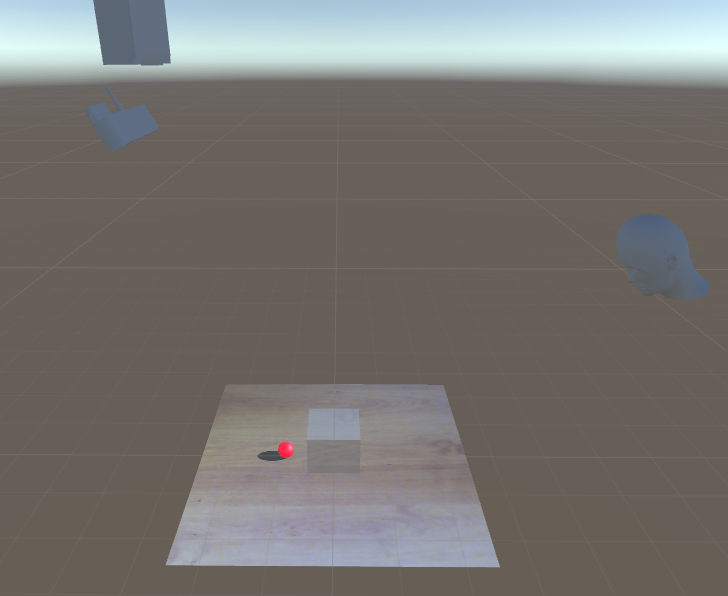
\includegraphics[width=0.65\linewidth]{images/unityscene}
\caption{Représentation du monde dans Unity - A droite la tête de l'utilisateur, au centre la table, en haut à gauche le couple caméra projecteur.}
\label{fig:unityrealworld}
\end{figure}

Le module \texttt{Unity} possède actuellement deux types de composants:
\begin{itemize}
\item Les composants modélisant les objets matériels du système de projection, correspondant aux différents dispositifs d'acquisition (caméras, projecteurs).
\item Les composants modélisant la partie logicielle, correspondant aux divers services de traitement fournis par \texttt{Nectar}
\end{itemize}

Le fonctionnement d'un composant, peu importe ce qu'il modélise, reste le même. Dans un premier temps, ce dernier créer un client et essaie de se connecter à la base de données Redis, base dans laquelle tous les services de \texttt{Nectar} si tant est qu'ils produisent des données stockent ces dernières. Si Redis n'est pas opérationnel et que la connexion échoue, il s'agit alors d'une erreur critique car cela signifie que \texttt{Nectar} n'a pas non plus pu démarrer ses services. Dans un tel cas, le composant envoie une requête HTTP au serveur web communiquant avec le gestionnaire de processus Eye dans le but de redémarrer Redis. Si Redis est toujours déconnecté, un message d'erreur critique est remonté à l'utilisateur qui ne pourra utiliser aucun des composants du module jusqu'à ce que Redis soit réparé. 
Une fois la connexion avec Redis établie, le composant, toujours par le biais d'une requête HTTP, questionne le serveur web sur l'état du service qu'il représente. Par exemple, le composant modélisant la caméra se renseignera sur l'état du service caméra. Si le service est hors ligne, une requête de démarrage peut être envoyée au serveur web qui la transmet instantanément à Eye afin de rendre opérationnel le service désiré. Si le service désiré n'existe pas, un message d'avertissement sur l'indisponibilité de ce dernier est remonté à l'utilisateur qui peut continuer à utiliser les autres composants du module.
Lorsque le service est démarré, ou s'il était déjà en ligne, le composant peut finalement récupérer les données qu'il désire dans Redis. Pour ce faire, ce dernier doit en connaître l'emplacement dans Redis. Redis fonctionnant sur un système de clé/valeur comme expliqué section~\ref{sec:nectararchi}, la connaissance a priori de la clé est nécessaire. C'est pourquoi chaque composant possède un ou plusieurs champs configurables par l'utilisateur pour indiquer les clés à utiliser pour récupérer les données dans Redis. Par exemple, le composant caméra qui doit à la fois récupérer les paramètres intrinsèques, extrinsèques et le format des données produites par la caméra possède trois champs configurables dans \texttt{Unity} permettant d'indiquer les clés de stockage dans Redis.

On peut observer, encadré dans la Figure~\ref{fig:unity:plugin}, les trois points importants du module. 
En vert est représentée la zone où les composants nécessaires à la création d'application sont ajoutés afin d'en utiliser les fonctionnalités. Ici par exemple, nous utilisons une caméra, un projecteur et une caméra de profondeur rangés dans la catégorie \emph{hardware}, un point de vue utilisateur \emph{UserPOV (Point Of View)} et différents services comme par exemple le suivi de feuille \emph{Paper Tracker}. Nous avons aussi ajouté à cette scène différents \emph{Renderer} permettant de visualiser les données acquises/générées par les dispositifs d'acquisition comme la caméra, le projecteur et la caméra de profondeur.
Ensuite, encadrée en rouge, on retrouve la zone où il va être possible de contrôler l'état des composants et, si besoin, de démarrer les services comme mentionné précédemment. Dans notre exemple, toujours Figure~\ref{fig:unity:plugin}, on observe le script de contrôle du composant projecteur. Ce script permet de spécifier quel type de dispositif on souhaite créer, ici la valeur est \emph{PROJECTOR}, on peut également voir l'état interne du composant, ici le composant est dans l'état \emph{WORKING}, ce qui signifie que ce dernier a réussi à se connecter à Redis, et à récupérer les données dont il avait besoin pour fonctionner, les clefs où sont stockées lesdites données à récupérer, et un bouton permettant de démarrer/redémarrer le service en cas d'échec lors de l'initialisation.
Enfin, encadrée en bleu, on peut voir la zone où les notifications de tout type (erreur, avertissement, fonctionnement) sont remontées à l'utilisateur lui indiquant constamment l'état des services et les problèmes détectés. Chaque notification commence par le nom du composant la générant suivi du message, afin de garder une certaine lisibilité.

\begin{figure}[H]
\centering
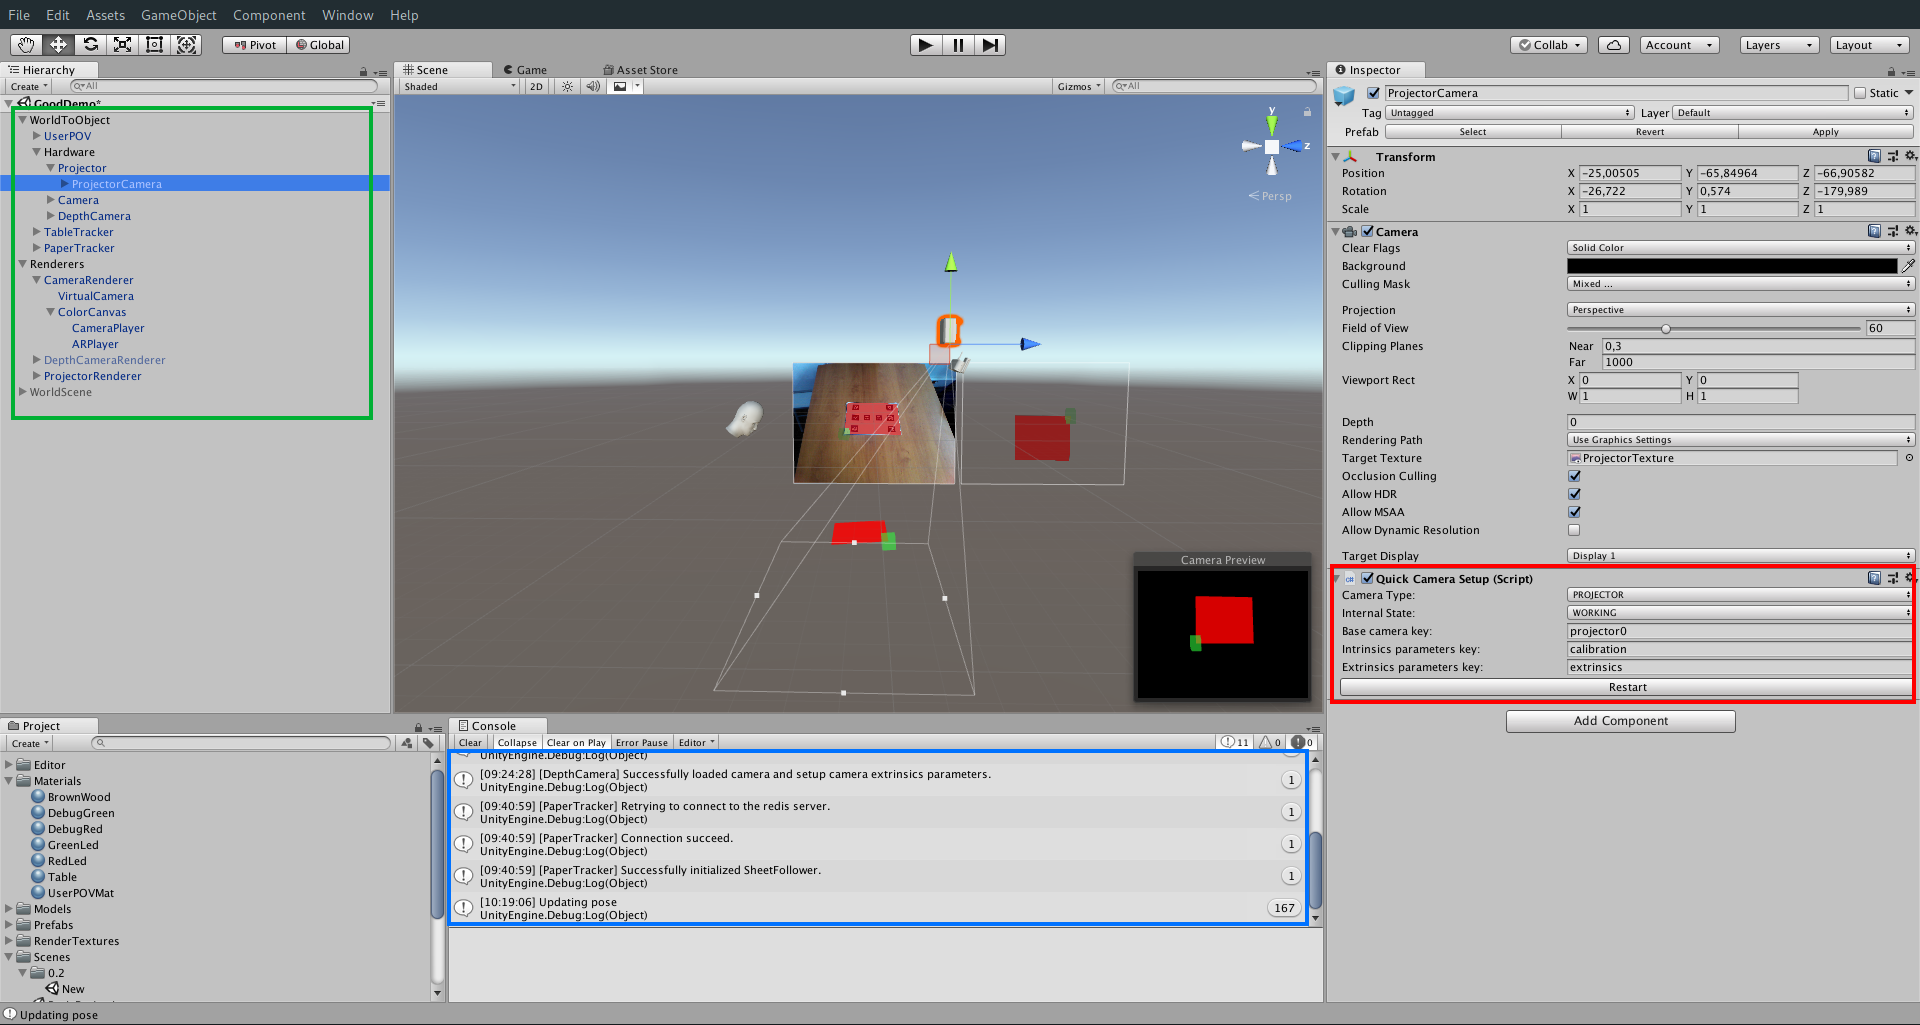
\includegraphics[width=\linewidth]{images/unity-plugin}
\caption{Vue globale du module Unity et de ses différents composants}
\label{fig:unity:plugin}
\end{figure}

Tous les composants et scripts ont été spécialement créé pour s'exécuter directement dans l'éditeur Unity afin de faciliter considérablement le développement pour les utilisateurs. Ainsi il n'est pas nécessaire de construire et d'exécuter l'application pour pouvoir avoir un retour sur la création en cours. Cela permet aussi de gagner en temps précieux et donc d'accélérer le développement.

Le mode éditeur possède cependant quelques défauts majeures qui ont requit une modification à la fois du module et à la fois des services Nectar afin qu'il fonctionne correctement. 
En effet, à l'origine les services Nectar utilisaient le pipeline événementiel de Redis pour qu'ils n'aient pas besoin d'effectuer de l'attente active et ainsi consommer 99\% des ressources, attendant infiniment de nouvelles données. Ce pipeline permettait de souscrire à certaines clés, pour être notifié lorsque des nouvelles données étaient poussées sur ces dites clés. Ce pipeline était très performant mais a posé quelques problèmes avec le fonctionnement en éditeur de \texttt{Unity}. En effet, en mode éditeur, les performances de \texttt{Unity} sont très amoindri\footnote{\href{https://forum.unity.com/threads/low-performance-in-editor-but-working-fine-in-build.489030/}{Unity : Low performance in editor}} et ce dernier n'était donc pas capable de traiter suffisamment vite les événements reçu. Les données s'accumulaient sans être consommées par les clients. Redis stockant ces données directement dans la mémoire vive comme expliqué section ~\ref{sec:nectararchi}, l'accumulation des celles ci causait une surcharge et mettait en péril toute la base. Il était donc nécessaire de couper la connexion avec le client du composant se trouvant dans l'incapacité de consommer ces données.

Pour que cette version puisse fonctionner correctement, nous avons décidé d'ajouter à tous les services Nectar la possibilité ou non d'utiliser le pipeline événementiel. Cette option permet donc d'utiliser le pipeline classique où les données ne s'accumulent pas mais écrase les anciennes déjà existantes. Du côté du module, le même comportement a été implémenté pour tous les composants fonctionnant directement dans l'éditeur afin de pouvoir utiliser les services. Cette solution résous bel et bien le fonctionnement en éditeur mais comporte encore quelques défauts.

Le pipeline ne se basant plus sur des événements, la seule façon de mettre à jour les composants est d'utiliser la boucle principale gérée par \texttt{Unity}. De ce fait, comme on peut le voir dans l'ordre d'exécution des différentes fonctions de \texttt{Unity} que vous trouverez en Annexe 3, celle de la boucle que nous pouvons utilisé sont celles de mise à jour (\emph{Update}). Le problème avec ces fonctions réside dans le fait que, lors de l'utilisation dans l'éditeur, celles ci ne sont pas systématiquement appelées, comme elles le seraient en mode jeu ou quand l'application est construire puis exécutée, afin d'alléger la consommation des ressources et permettre d'avoir un meilleur confort lors de développement. Ainsi, il en résulte que actuellement les composants ne se mettent à jour que lorsque \texttt{Unity} reçoit des événements et décide de se mettre à jour comme c'est le cas si une valeur telle que la position d'un objet est modifiée.\\

Une des dernières difficultés rencontrée durant le développement du module Unity a été la gestion des formats de données envoyés par les différents services et plus spécifiquement les matrices. Chaque service étant indépendant les données qu'il envoi ne sont pas toujours au même format que celui attendue par Unity. En effet, si on prends le cas des matrices, celles du moteur 3D de Unity sont dites \emph{row major} ce qui signifie que les données sont indexés en fonction des lignes alors que celle du moteur 3D de Processing sont dites\emph{column major}, et donc en fonction des colonnes. Il a donc fallut appliquer des traitements spécifiques en fonction des données reçu afin d'obtenir une visualisation cohérence de ces dernières.

Une fois la majeur partie des problèmes du module résolue, il était temps d'enfiler le costume d'utilisateur développeur client de \texttt{RealityTech} et d'expérimenter le développement d'une application de réalité augmentée spatiale avec ce module. Vous trouverez les détails de ce développement section~\ref{sec:unity:appli}.

\section{Illusion de projection}
\label{sec:unity:appli}

Après voir achever la première version du module Unity, dans une optique de test de ce dernier mais aussi dans le but de proposer une preuve de concept, j'ai été charger de développer une application utilisant une illusion de projection afin de créer un effet de fausse transparence. Cette preuve de concept avait été demandé par des potentiels clients de la société rencontrés au Laval Virtual, afin qu'ils puissent effectuer de la présentation de produit interactive, et plus spécifiquement de la présentation de parfum. C'est typiquement un cas d'utilisation auquel il était très difficile de répondre avec la version \texttt{Processing} du kit de développement car elle ne permettait pas facilement de manipuler des objets 3D, de gérer la transparence, de faire le rendu de la scène en plusieurs étapes etc... . 

Afin de pouvoir créer une illusion de projection, il est nécessaire d'avoir une connaissance a priori de la surface de projection, permettant d'appliquer les déformation nécessaire à la géométrie a projeter. Grâce à la représentation du monde réel directement dans \texttt{Unity}, nous pouvons aisément disposer des éléments de géométrie qui nous sont nécessaire Figure~\ref{fig:realvsunity}. Ainsi, seuls les éléments purement virtuels à projeter sont à rajouter dans la scène 3D.

\begin{figure}[H]
\centering
	\subfloat[Photographie de la scène]{
      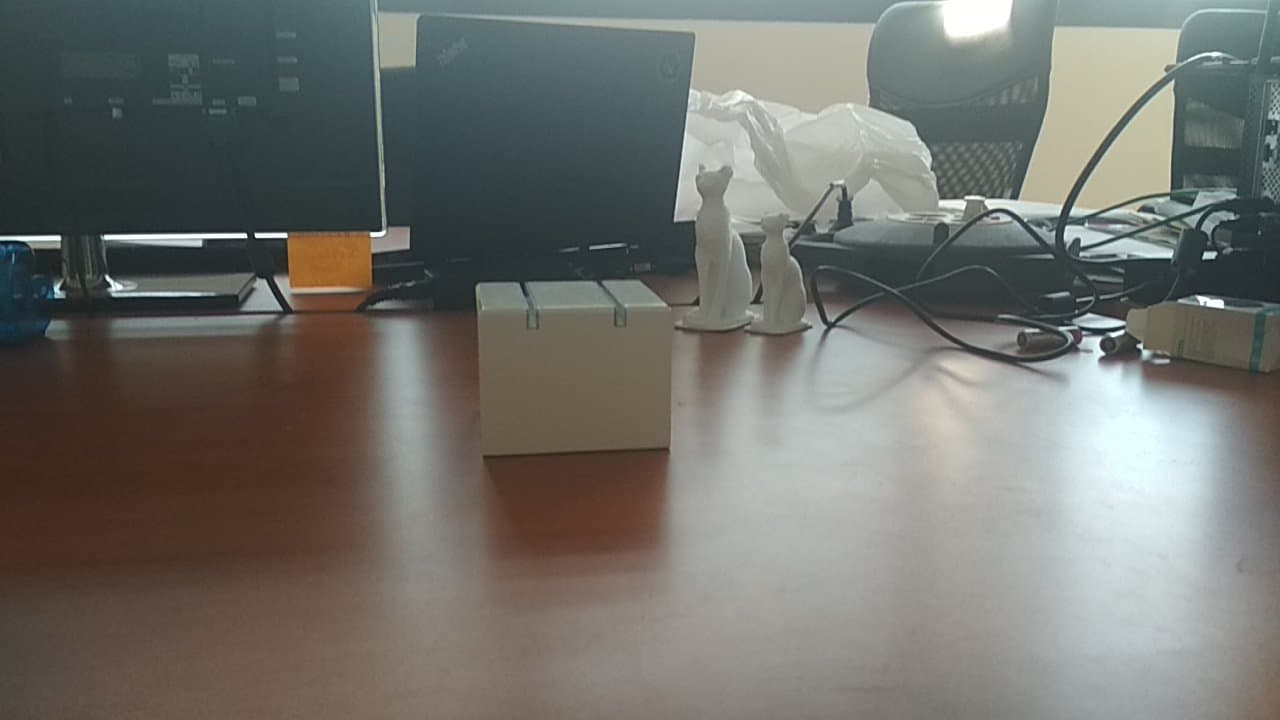
\includegraphics[width=0.45\textwidth, trim = 7.5 2.5cm 7.5cm 5cm, clip]{images/Unity-Projection-RealReal}
      \label{sub:unity:app:realworldview}
      }
     \subfloat[Représentation dans Unity]{
      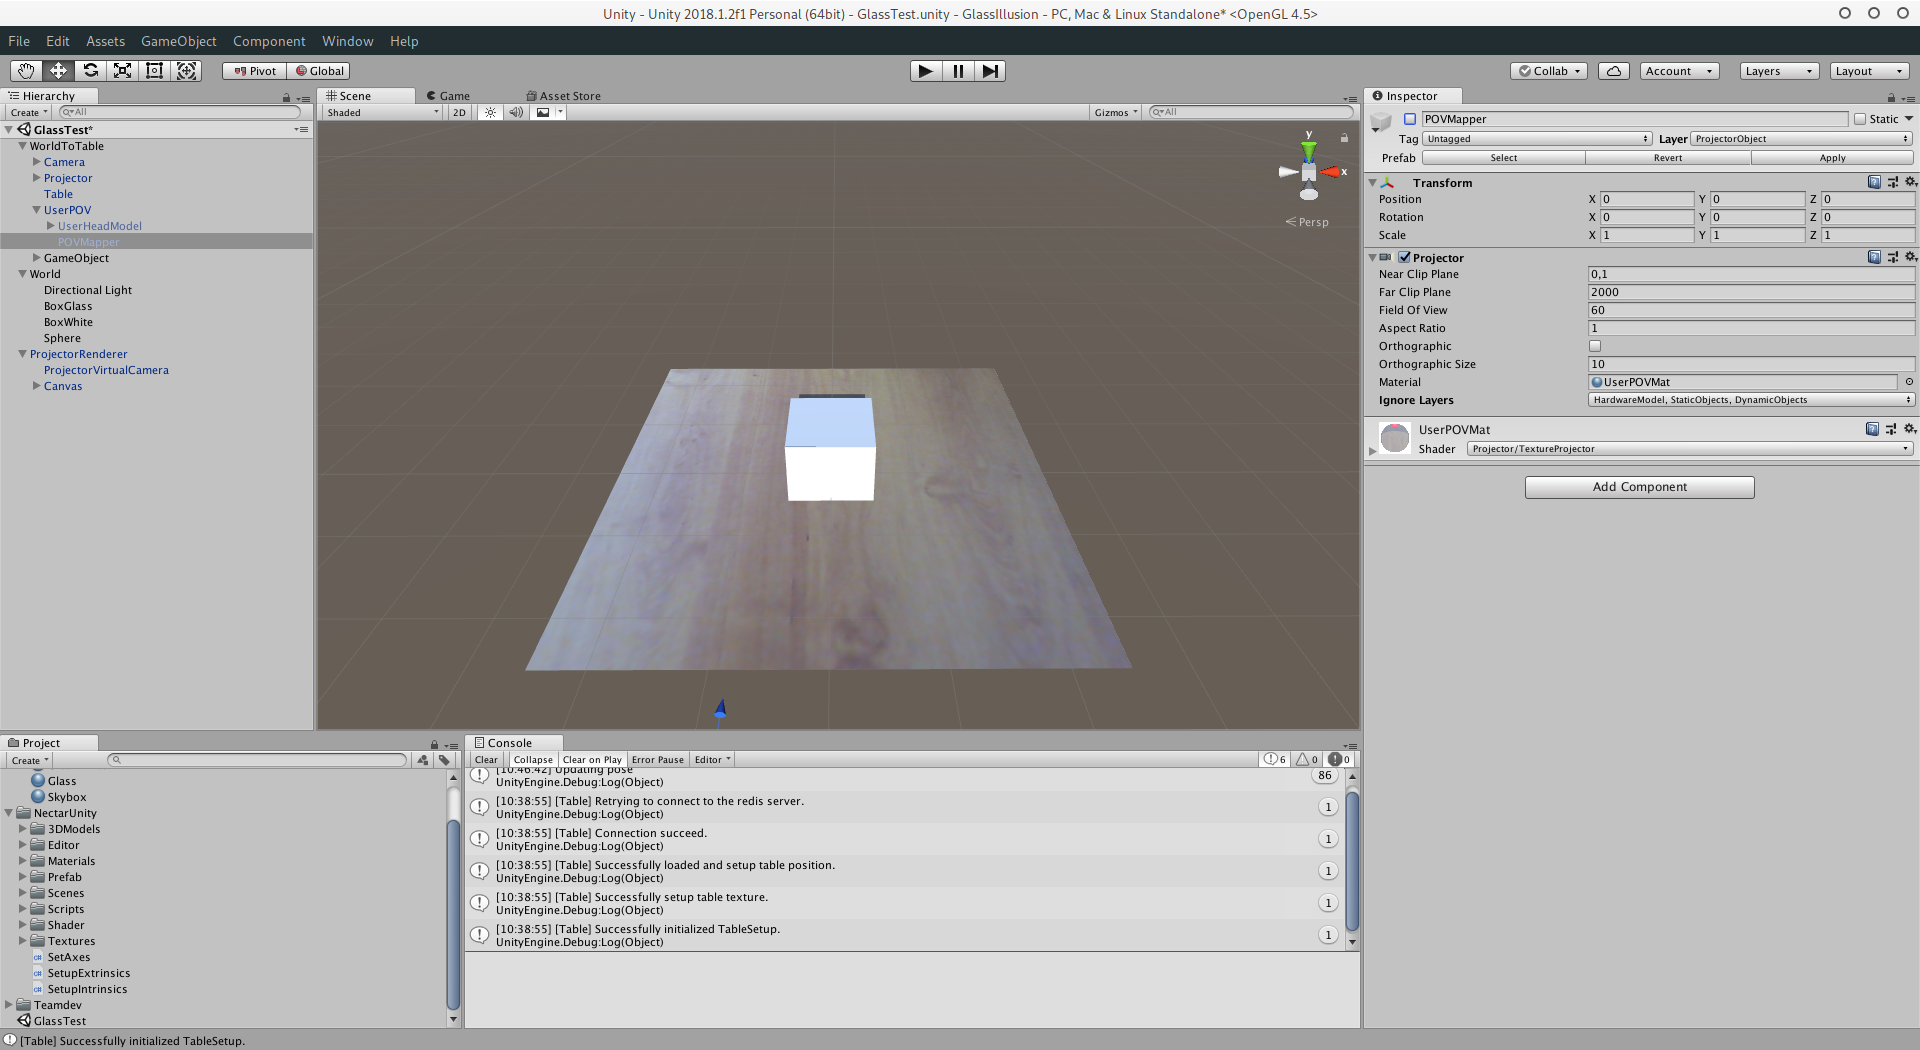
\includegraphics[width=0.45\textwidth, trim = 12cm 12cm 20cm 4.5cm, clip]{images/Unity-Projection-UserPOV-NoMap}
      \label{sub:unity:app:unityview}
      }
\caption{Monde réel et sa représentation dans Unity}
\label{fig:realvsunity}
\end{figure}

Aussi, une illusion de projection ne fonctionne que pour un point de vue donnée Figure~\ref{fig:projpov} car la perception de la géométrie du monde réel diffère selon ce dernier ce qui signifie que les déformations à appliquer ne seront donc pas les mêmes.

\begin{figure}[H]
\centering
	\subfloat[Bon point de vue] {
	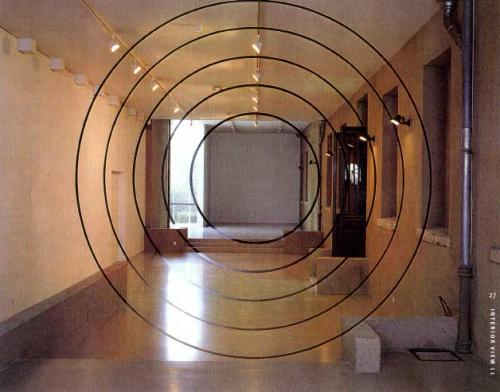
\includegraphics[width=0.45\textwidth]{images/proj-illu-good-pov}
	\label{sub:ilu:badpov}
	}
	\subfloat[Mauvais point de vue] {
	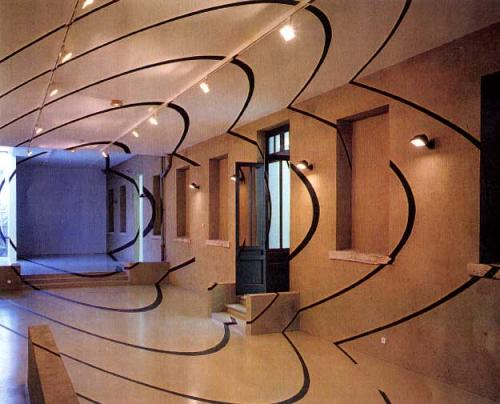
\includegraphics[width=0.42\textwidth]{images/proj-illu-bad-pov}
	\label{sub:ilu:goodpov}
	}
\caption{Illusion de projection}
\label{fig:projpov}
\end{figure}

Ainsi les éléments requis pour commencer a créer notre illusions sont: la modélisation du monde réel, ici la table, sa texture (pour que l'effet de transparence ait du sens), et le flacon de parfum que l'on souhaite faire apparaître transparent, la position de l'utilisateur observant la scène et le point de vue du projecteur. Tous ces éléments font partie du module de développement il a donc suffit de les ajouter a la scène pour en obtenir la représentation Figure~\ref{fig:unity:projscene}.
Afin de vérifier la validité de l'effet, nous avons aussi choisit d'ajouter une sphère virtuelle rouge derrière le flacon, invisible du point de vue de l'utilisateur, de façon a ce qu'elle appairasse lorsque l'effet de transparence sera mis en place.

\textbf{Note:} Dans notre cas, nous n'avions pas le modèle 3D du parfum imprimé à disposition, nous avons donc choisit de le remplacer par un cube cependant cela n'a aucun impact sur la simulation de l'effet de transparence.

\begin{figure}[H]
\centering
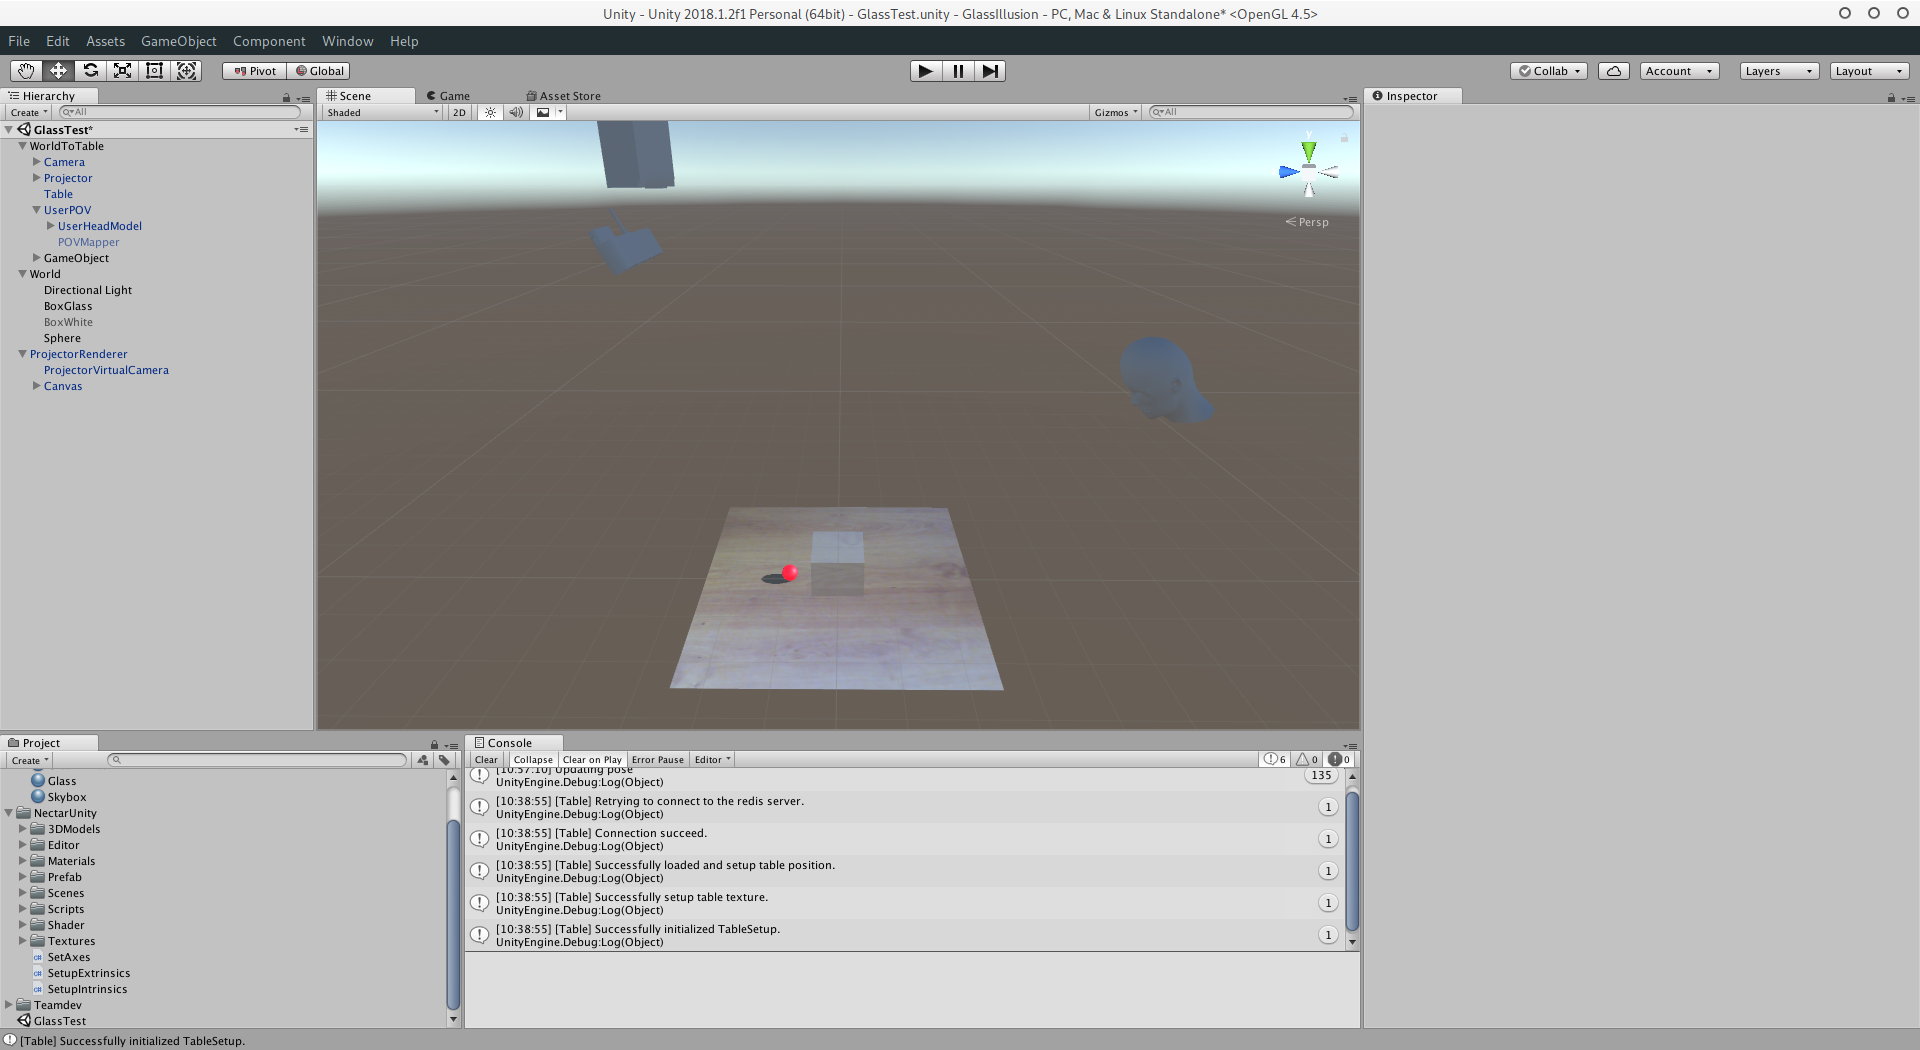
\includegraphics[width=0.75\linewidth, trim = 12cm 12cm 20cm 4.5cm, clip]{images/Unity-Projection-RealScene}
\caption{Scène modélisée pour tester l'effet de transparence}
\label{fig:unity:projscene}
\end{figure}

Pour réaliser un tel effet, le rendu se fait en plusieurs étapes. Dans un premier temps, le rendu de la scène est effectué depuis le point de vue de l'utilisateur avec l'objet d'intérêt transparent et en ignorant sa représentation physique Figure~\ref{sub:unity:proj:userpov:transparency}. Ce rendu se fait offscreen et est ensuite récupéré dans une texture. C'est cette texture qui subira les déformations afin d'être projeté sur la géométrie et de créer l'illusion. La prochaine étape du rendu consiste justement à utiliser la texture ainsi créée et à la projeter sur la géométrie de la scène comprenant cette fois ci l'objet physique afin de créer l'illusion Figure~\ref{sub:unity:proj:userpov:nomap},~\ref{sub:unity:proj:nopov:map} et~\ref{sub:unity:proj:userpov:map} . On peut observer qu'une ombre est apparu, en effet, pour renforcer l'effet qu'allait produire l'illusion nous avons choisit d'ajouter une lumière afin d'obtenir des ombres cependant nous avons oublier d'activer leur rendu pour les objets transparents. Pour pouvoir projeter cette texture sur la scène il a fallut implémenter un principe de vidéo projecteur. Ce vidéo projecteur ne devait projeté la texture cette fois ci que sur le modèle physique et pas sa représentation transparente.
Enfin la dernière étape consiste a finalement faire le rendu de la scène, avec la texture projetée sur la géométrie vu par le projecteur Figure~\ref{sub:unity:proj:projectorpov:map} pour ainsi pouvoir projeter ce résultat dans le monde réel. Je n'ai malheureusement pas eu l'occasion de prendre une photo de ce dispositif entrain de fonctionner.
\begin{figure}[H]
\centering
	\subfloat[Point de vue utilisateur - Objet transparent] {
		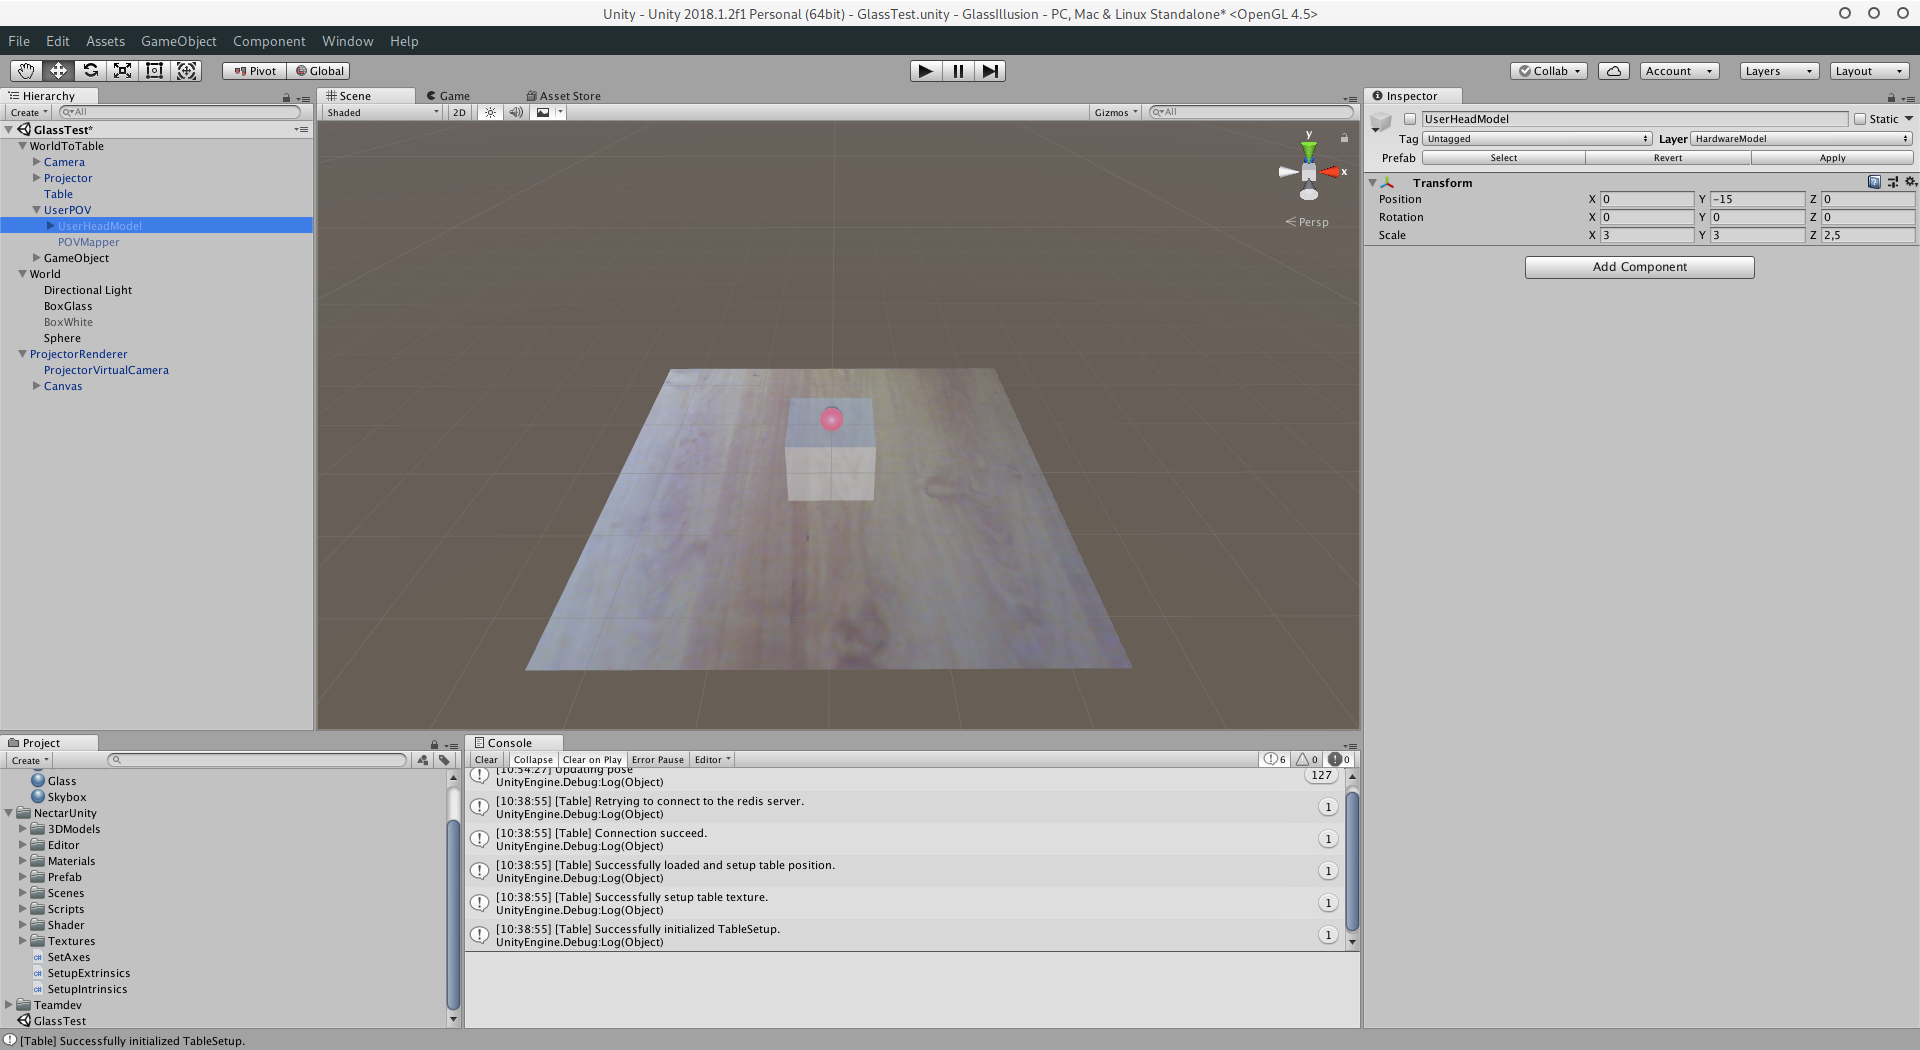
\includegraphics[width=0.4\textwidth, trim = 12cm 12cm 20cm 4.5cm, clip]{images/Unity-Projection-UserPOV-RealScene}
		\label{sub:unity:proj:userpov:transparency}
	}
	\subfloat[Point de vue utilisateur - Objet physique] {
		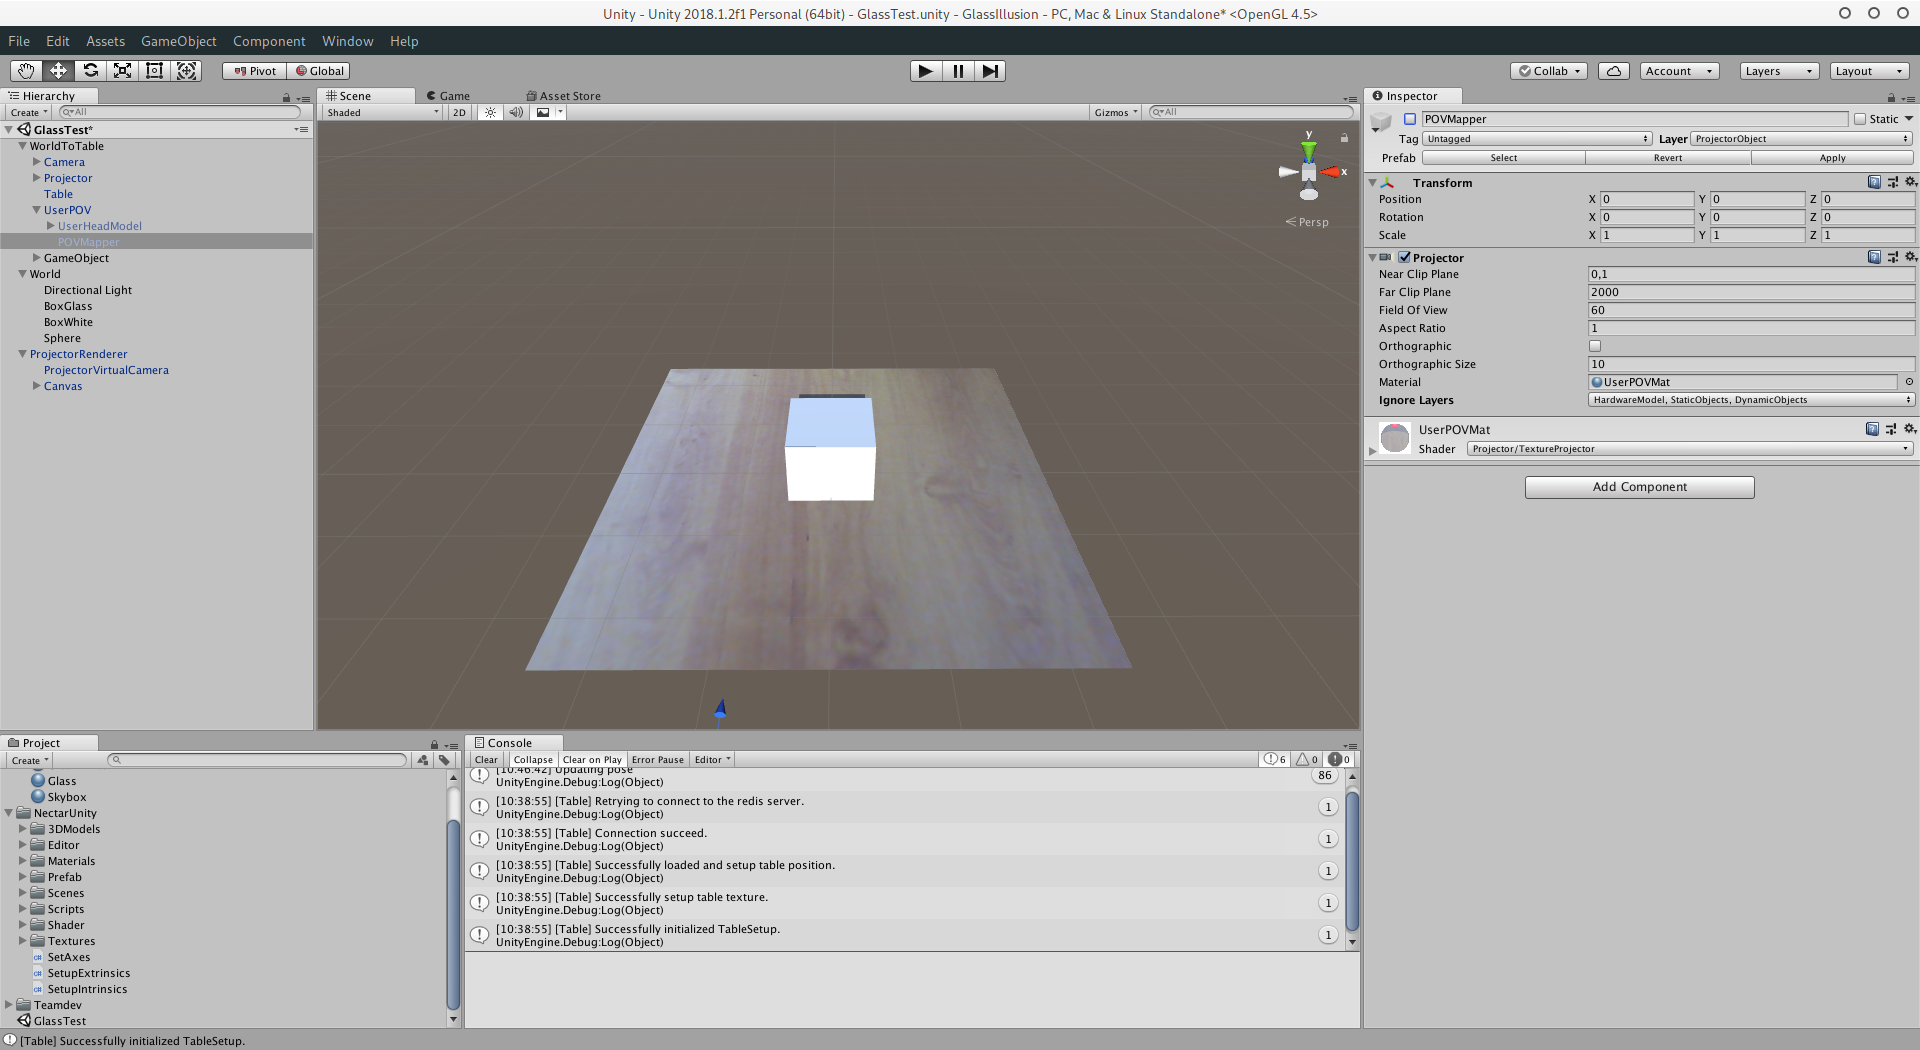
\includegraphics[width=0.4\textwidth, trim = 12cm 12cm 20cm 4.5cm, clip]{images/Unity-Projection-UserPOV-NoMap}
		\label{sub:unity:proj:userpov:nomap}
	}\\
	\subfloat[Point de vue différent - Objet physique + texture projetée] {
		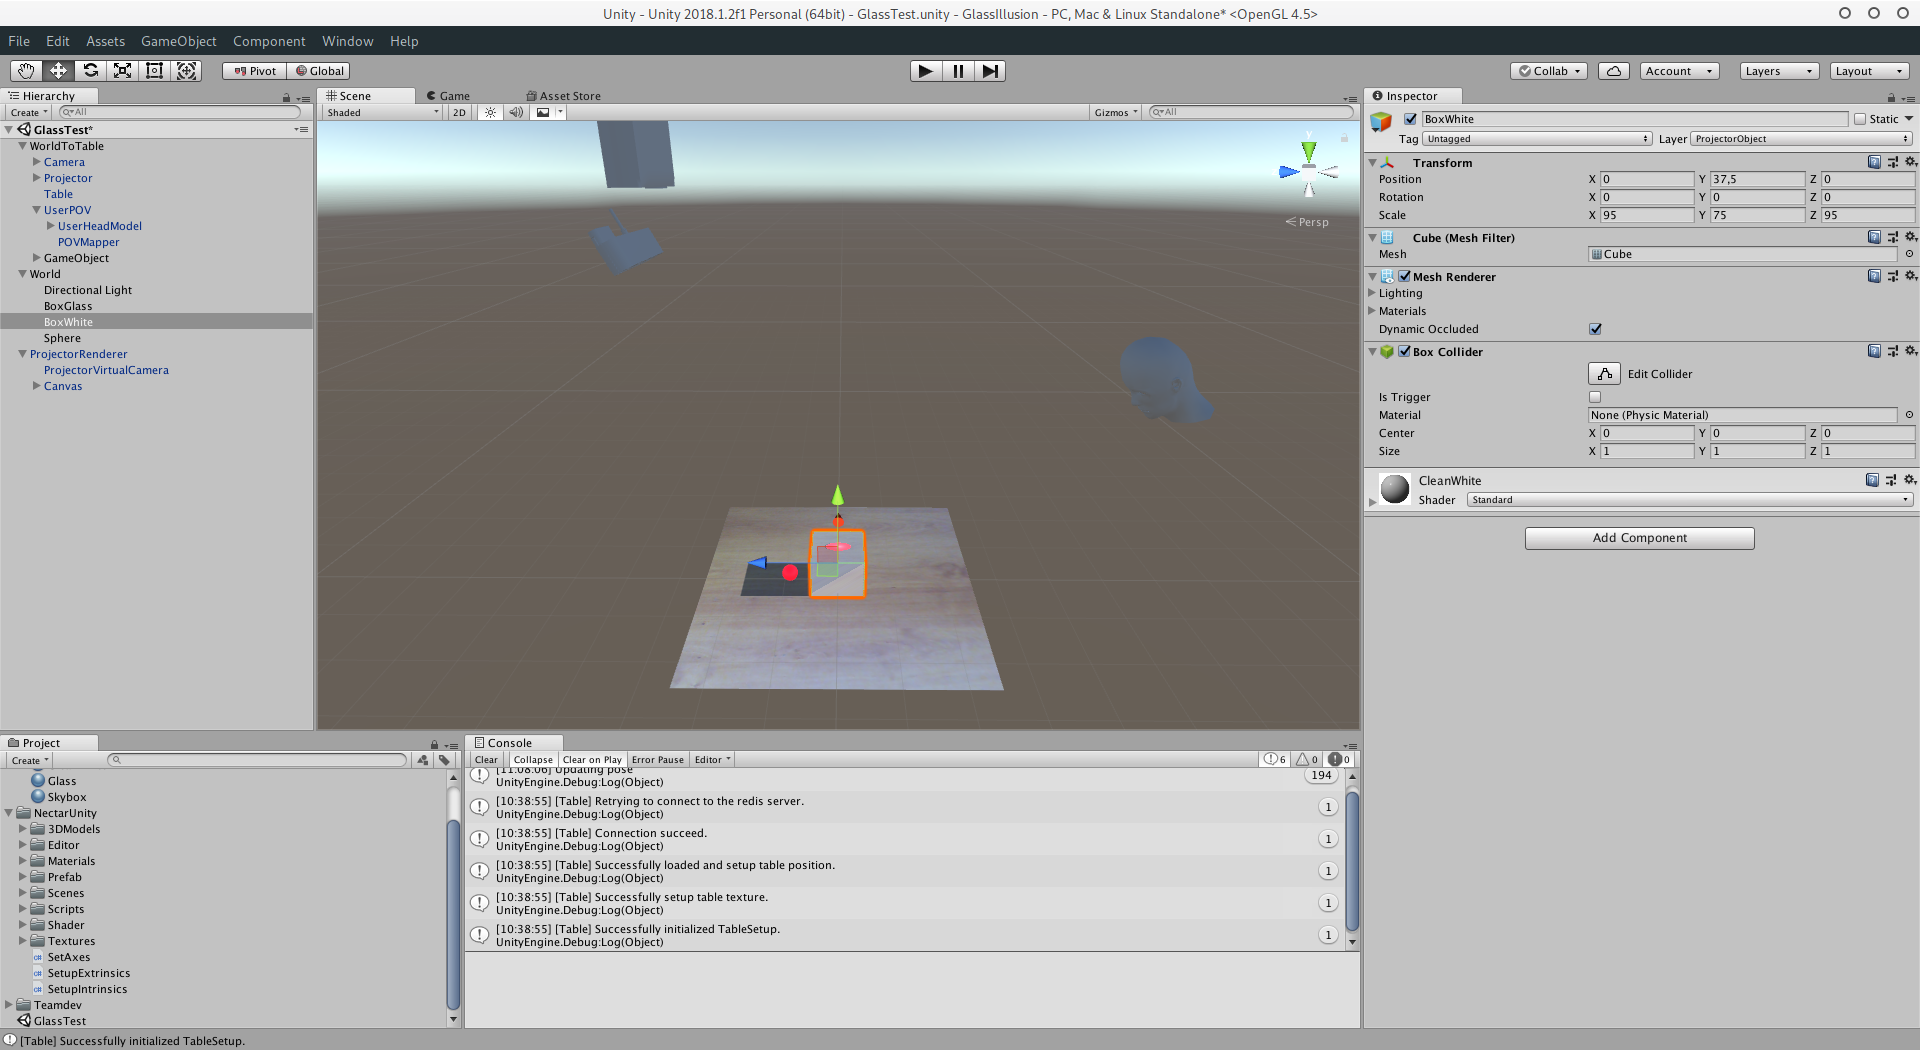
\includegraphics[width=0.4\textwidth, trim = 12cm 12cm 20cm 4.5cm, clip]{images/Unity-Projection-RealSceneWithMap}
		\label{sub:unity:proj:nopov:map}
	}
	\subfloat[Point de vue utilisateur - Objet physique + texture projetée] {
		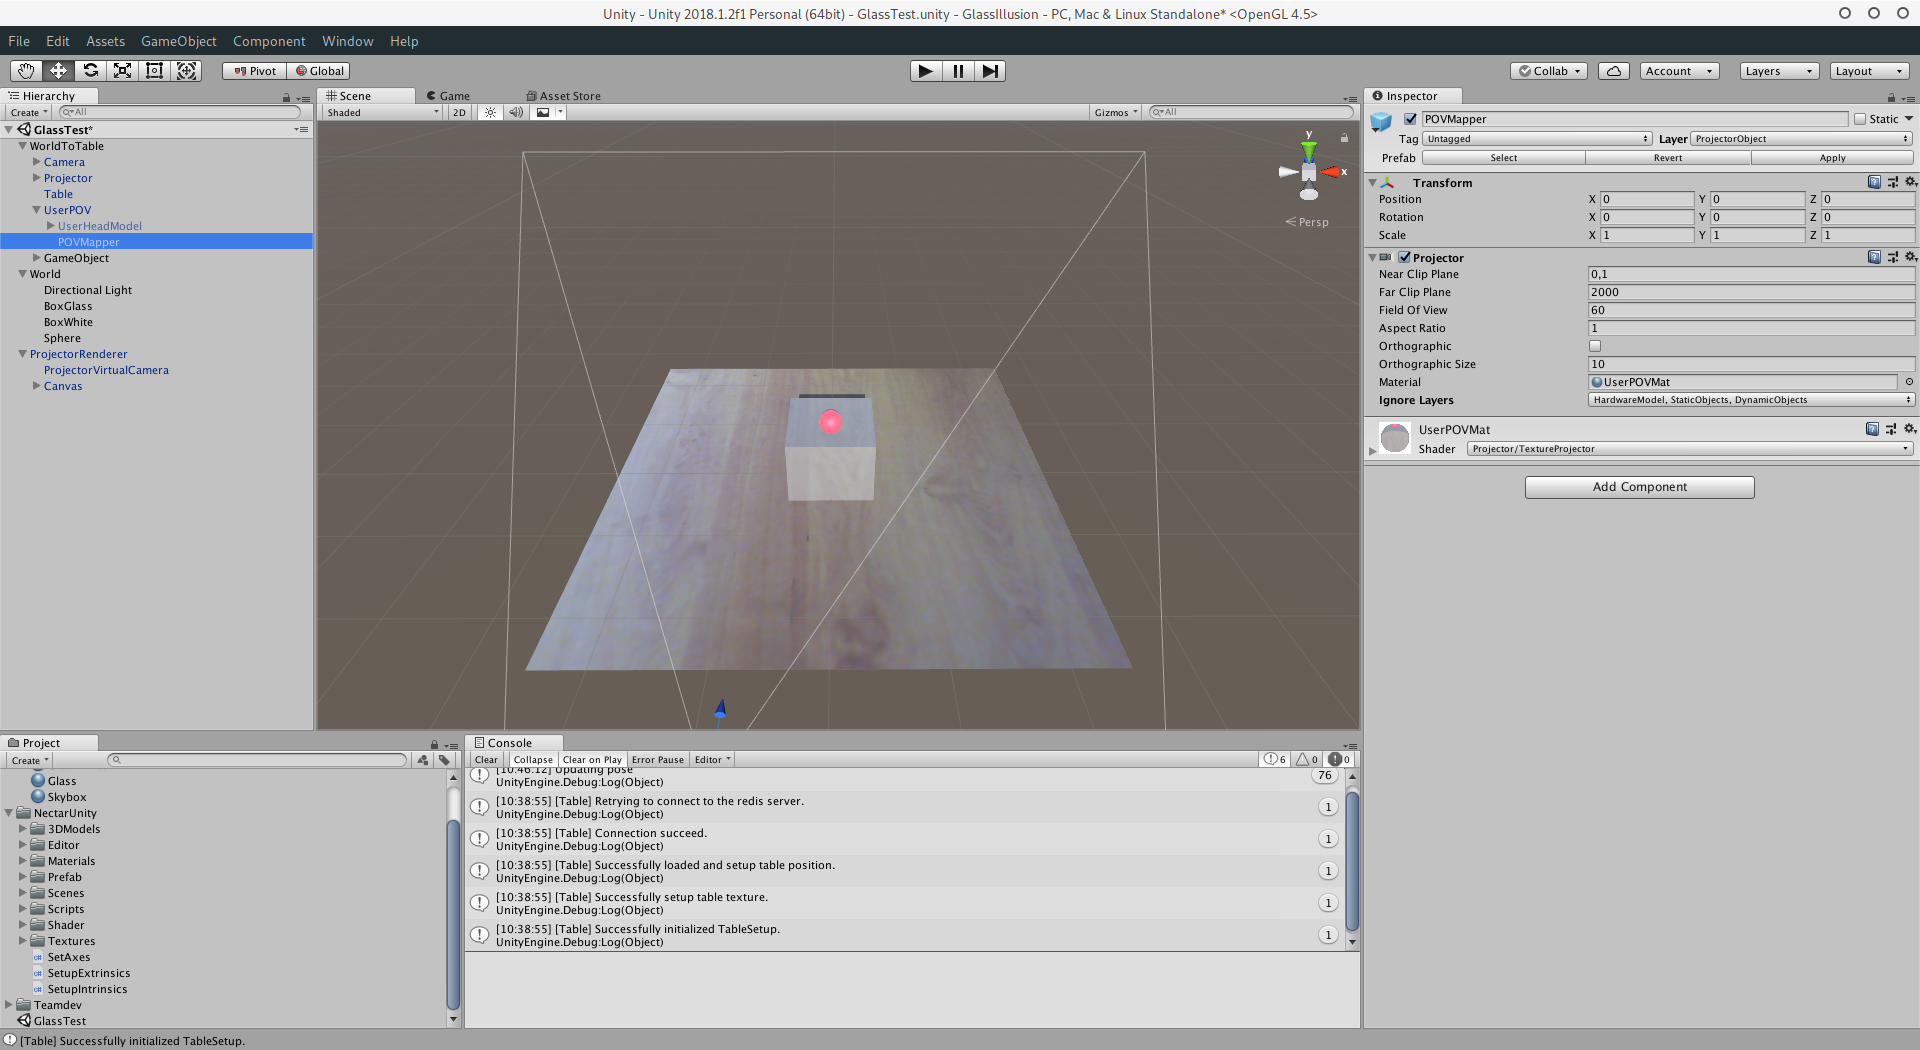
\includegraphics[width=0.4\textwidth, trim = 12cm 12cm 20cm 4.5cm, clip]{images/Unity-Projection-UserPOV-Mapper}
		\label{sub:unity:proj:userpov:map}
	}\\
	\subfloat[Point de vue projecteur - Objet physique + texture projetée] {
		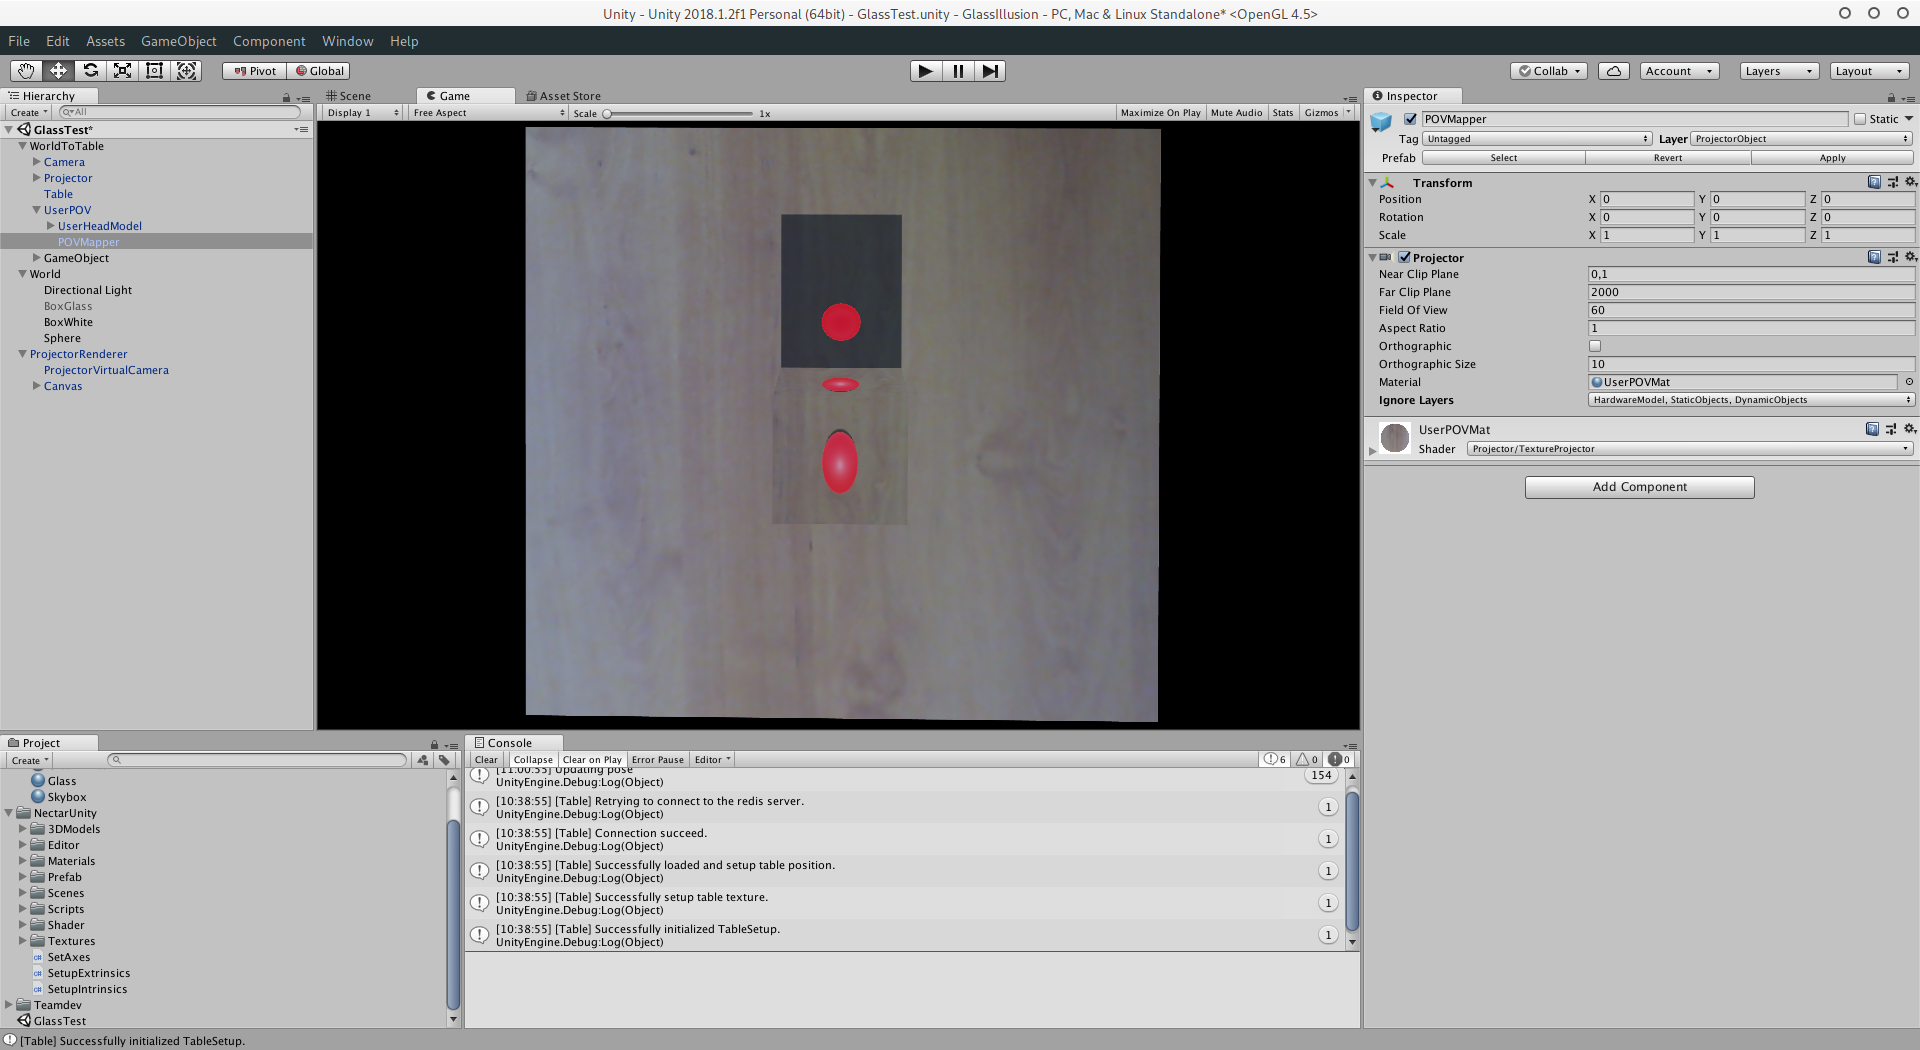
\includegraphics[width=0.4\textwidth, trim = 12cm 12cm 20cm 4.5cm, clip]{images/Unity-Projection-ProjectorPOV}
		\label{sub:unity:proj:projectorpov:map}
	}
\caption{}
\label{}
\end{figure}

Dans l'état actuel des choses, l'illusion est encore incomplète pour plusieurs raisons. La première étant que nous utilisons actuellement un système composé d'un seul projecteur. Il est, de ce fait, impossible de couvrir toute la surface du cube ou de n'importe quel objet en général avec de la projection. Aussi pour renforcer l'illusion, il aurai été intéressant d'utiliser la caméra ainsi que la caméra de profondeur du système pour créer des représentation 3D virtuelles des éléments du monde réel. Ces objets 3D aurait ainsi pu être intégré à la scène dans Unity et donc a l'illusion de transparence. De ce fait, si par exemple, une personne décidait de passer sa main derrière le cube physique non transparent dans le monde réel, il aurait été possible de lui afficher cette dernière en transparence derrière le cube.

\section{Bilan}
Comme on pouvait s'y attendre, le développement d'application de réalité augmentée spatiale avec Unity est très agréable. Le coût en développement (du module, de l'architecture en microservices etc.) est largement contrebalancé par les multiples possibilités offertes par ce moteur. De plus, le module répond assez bien aux objectifs que nous nous étions fixés que ce soit en termes de performance ou d'expérience pour l'utilisateur développeur.

Le fonctionnement en mode éditeur apporte un vrai plus dont nous avons pu ressentir l'effet lors du développement de l'application dont il est question section~\ref{sec:unity:appli}. Toutefois, la nécessité de générer des événements pour qu'Unity mettent à jour les composants reste pénible. Pour pallier à ce problème, nous avons imaginé une nouvelle version des microservices utilisant le pipeline évènementiel de Redis, où ces derniers ne publient plus les données qu'ils génèrent mais plutôt une notification au format json très légère, ne risquant donc pas de surcharger la RAM, et permettant d'indiquer aux services que des nouvelles données sont disponibles. On peut ainsi résoudre le problème de la surcharge mémoire et de l'attente active.

Par ailleurs, la gestion des clés pour accéder aux données dans le module est très peu pratique et en complexifie l'utilisation sans qu'il n'y ai aucun bénéfice pour l'utilisateur. Une solution à ce problème aurait été de supprimer la gestion des clés dans Unity et de l'exporter sur le serveur web. Ainsi, lors d'une requête de démarrage d'un service, le serveur web en plus de démarrer ce service, pourrait envoyer à Unity, une réponse contenant la clé où ce dernier publie ses données. La gestion des clefs deviendrait alors totalement invisible pour l'utilisateur du module ce qui lui permettrait de concentrer ses efforts sur le contenu de l'application.